\documentclass[12pt]{article}
\usepackage[margin=1in]{geometry}
\usepackage{graphicx}
\usepackage{alltt}
\begin{document}

\title{Clustering of Articles by Theme and Sentiment \\ {\Large Natural Language Processing Final Report}}
\author{Courtney Fiala and Anders Maraviglia}

\maketitle

\abstract{To objectively determine the semantic relationship between different selections of text has proven itself to be a difficult problem. Specifically, a computational method for identifying and quantifying the bias between news articles written on the same theme has yet to be implemented. Methods for sentiment and thematic extraction of textual articles have been previously explored. However, these algorithms have not been applied together in a comprehensive application to form any relationship between articles. We propose a novel solution that leverages natural language processing methods including theme extraction and sentiment analysis to graph a set of articles into clusters based on their themes and to convey the sentimental differences between articles. This can be applied to display a side-by-side comparison of two articles presenting opposing viewpoints on a specific theme.}

\section{Introduction}
There are many existing methods that classify articles based on broad themes and still more methods that determine the sentiment of a particular sentence. Most theme extraction algorithms classify an article into one of a predetermined set of classes, such as politics, sports, or weather. We wish to view more in-depth themes such as the most recent presidential debate or the championship basketball game. Further there exist a few websites that present a set of articles with opposing viewpoints on a particular subject, but these sites use hand-selected data instead of employing natural language processing methods.

A group of RCOS students is working on a project (Opinionated) to create a web application to display two news articles with differing viewpoints on a randomly generated theme. This group would like to use a computer algorithm to select which articles to display. There is currently no method to determine the themes of a set of articles then compare a pair of articles based on their sentiments towards one theme.

Our goal this semester was to create an in-depth theme extraction and sentiment analysis approach for the article clustering. This approach was to be exported into a module that can be used by the Opinionated team in their application to generate the relationship between article viewpoints.

\section{Approach}
Our approach focused on two main areas: (1) theme extraction and sentiment analysis and (2) link creation.

During the theme extraction step, we began with a set of news articles marked by hand with their themes and sentiments. For each of these articles, we extracted sentence-level analysis data using IBM's Alchemy API. We then aggregated the sentence data into a single dataset for each article using a weighted average. The descriptions of the extracted data can be seen in Table 1.

During aggregation, article sentiment and emotion were found by performing a weighted average of the sentiment and emotion levels extracted for each sentence and for each entity and keyword. Averages were weighted using relevance scores.

In order to form links between articles, a set of comparison functions was created to determine the relationship between two articles. First, the relationship between the themes of articles was found by comparing the articles' entities, keywords, and taxonomies. A weighted average was performed, calculating the number of matched entities and keywords compared to the total number of entities and keywords found in both articles. Upon tweaking the weight used in this average, we found that 1+relevance achieved the best results. This was similarly applied for taxonomies. If two articles were found to have similar themes, a we created a link between them then evaluated their sentimental and emotional relationship.

The relationship between the viewpoint of two articles was calculated by aggregating the maximum emotional difference and the difference in sentiments. If two articles' viewpoints were sufficiently different, the link between the articles was labeled as containing ``opposing'' viewpoints. On the other hand, if the differences between these articles was insufficient, the link was labeled as ``similar''.

When the link creation was complete, we formed a visualization of the article relationships in the form of a graph. Each article is a node containing its keywords, entities, and taxonomy; each edge represents a thematic relationship and is correspondingly labeled as either ``similar'' or ``opposing'' based on the viewpoint relationship aggregation.

\begin{table}
	\begin{tabular}{|l|l|}\hline
		Feature & Description\\\hline
		Entities & List of entities extracted using named-entity recognition\\
		Keywords & List of keywords extracted\\
		Relevance & Relevance of an entity or keyword in a sentence\\
		Taxonomy & 5-level categorical theme extraction with a corresponding weight\\
		Sentiment & Positive, Neutral, or Negative with a corresponding weight\\
		Emotions & Weights for levels of Anger, Joy, Fear, Sadness, and Disgust\\\hline
	\end{tabular}
	\caption{Description of all features used in article comparison. Note that Sentiments and Emotions were found sentence-level as well as word-level for entities and keywords.}
\end{table}

\section{Experiments}
The majority of the experimentation performed during this project was to determine the weights and thresholds used during aggregation steps. First, we found the proper weighting scheme for aggregating sentiment and emotion by evaluating the $F_1$-score of multiple weights. Out of a combination of baseline, frequency, and relevance weights, we found that relevance gave the best results. Similarly, we evaluated the proper threshold to be used for each of the comparisons: (1) entities and keywords, (2) taxonomy, (3) sentiment, and (4) emotion. For conciseness, we have only included the final results for all thresholds in Table 2.

\begin{table}
	\begin{tabular}{|c|c|c|c|c|}\hline
		 & Entites/Keywords & Taxonomy & Sentiment & Emotion\\\hline
		Threshold & 0.06 & 0.25 & 0.12 & 0.12\\\hline
	\end{tabular}
	\caption{Final threshold values for each comparison during link creation}
\end{table}

\section{Results}
Upon completion of our project, we have both a file format and a visualization of the linked articles. The visualization is a graph representation of the links between articles. Nodes that contain links are clustered together. Nodes and edges can be expanded to display article and relationship information. Screenshots of the article graph and a sample individual article node from the interactive visualization can be found in the appendix. Note that article viewpoints are displayed on the edges.

Our file output is in JSON format, and contains a list of all linked articles along with their entity, taxonomy, sentiment, and emotion comparison scores and a viewpoint indicator. An example article link is shown below:
\begin{alltt}
\{
  article 1: GovChristieLeavesGunControlsBehindinNewJersey
  article 2: RepublicanCandidatesDeeplyEntrenchedAgainstGunControls
  entity:    0.0859298046379
  taxonomy:  0.312259510317
  sentiment: 0.167339384365
  emotion:   0.117104697335
  viewpoint: similar
\}
\end{alltt}

\section{Discussion}
We have reached our baseline goal to develop both 
\begin{itemize}
\item A visual representation of article relationships, in the form of a graph with articles as nodes and edges representing relations between articles
\item A file-based representation of the relationships between articles, which can be easily imported and parsed by another program.
\end{itemize}
We did not meet our stretch goals to extend our module further. We wished to extract the organizations and people mentioned in an article and determine each entity's viewpoint on the article topics. Thus given a set of articles, we can determine the general viewpoints of any particular organization mentioned across the entire set.

In the future, we will continue to develop our module in order to incorporate our stretch goals. While these features may not be used by the Opinionated group, we feel they can be utilized in developing more robust comparisons between different organizations as seen by the media. For example, this could be useful in extracting the viewpoints of a political party on the topic of building an oil pipeline, or a similar development. We also wish to develop a more advanced visualization of the article links. For example, links that change the edge width based on the strength of a relationship.

\section{Appendix}
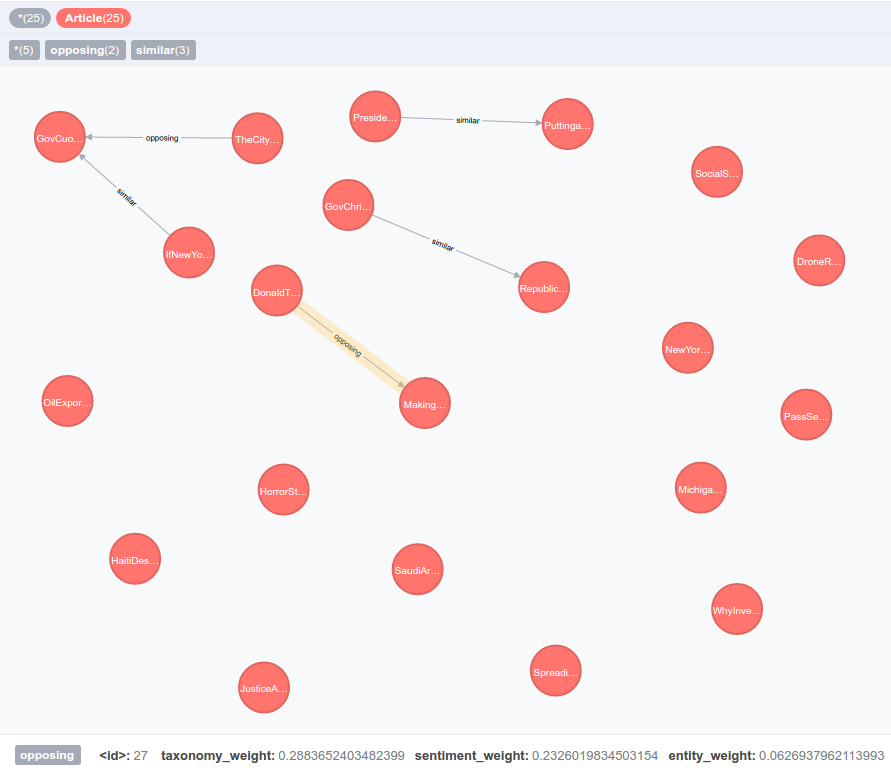
\includegraphics[width=5.75in]{graph_screenshot}
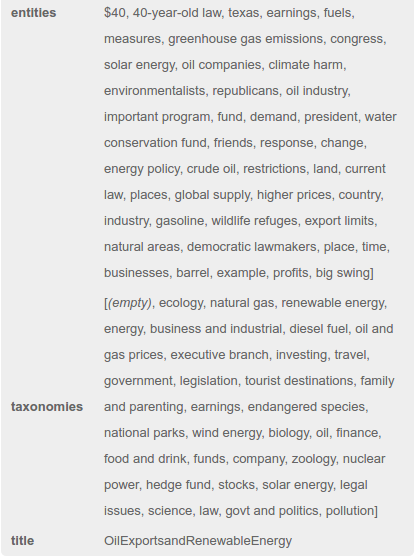
\includegraphics[width=3in]{graph_node_screenshot}

\end{document}
